\documentclass[]{elsarticle} %review=doublespace preprint=single 5p=2 column
%%% Begin My package additions %%%%%%%%%%%%%%%%%%%
\usepackage[hyphens]{url}

  \journal{Journal of Transport Geography} % Sets Journal name


\usepackage{lineno} % add
\providecommand{\tightlist}{%
  \setlength{\itemsep}{0pt}\setlength{\parskip}{0pt}}

\usepackage{graphicx}
\usepackage{booktabs} % book-quality tables
%%%%%%%%%%%%%%%% end my additions to header

\usepackage[T1]{fontenc}
\usepackage{lmodern}
\usepackage{amssymb,amsmath}
\usepackage{ifxetex,ifluatex}
\usepackage{fixltx2e} % provides \textsubscript
% use upquote if available, for straight quotes in verbatim environments
\IfFileExists{upquote.sty}{\usepackage{upquote}}{}
\ifnum 0\ifxetex 1\fi\ifluatex 1\fi=0 % if pdftex
  \usepackage[utf8]{inputenc}
\else % if luatex or xelatex
  \usepackage{fontspec}
  \ifxetex
    \usepackage{xltxtra,xunicode}
  \fi
  \defaultfontfeatures{Mapping=tex-text,Scale=MatchLowercase}
  \newcommand{\euro}{€}
\fi
% use microtype if available
\IfFileExists{microtype.sty}{\usepackage{microtype}}{}
\bibliographystyle{elsarticle-harv}
\usepackage{graphicx}
% We will generate all images so they have a width \maxwidth. This means
% that they will get their normal width if they fit onto the page, but
% are scaled down if they would overflow the margins.
\makeatletter
\def\maxwidth{\ifdim\Gin@nat@width>\linewidth\linewidth
\else\Gin@nat@width\fi}
\makeatother
\let\Oldincludegraphics\includegraphics
\renewcommand{\includegraphics}[1]{\Oldincludegraphics[width=\maxwidth]{#1}}
\ifxetex
  \usepackage[setpagesize=false, % page size defined by xetex
              unicode=false, % unicode breaks when used with xetex
              xetex]{hyperref}
\else
  \usepackage[unicode=true]{hyperref}
\fi
\hypersetup{breaklinks=true,
            bookmarks=true,
            pdfauthor={},
            pdftitle={Comparing distance, time, and metabolic energy cost functions for walking accessibility in infrastructure-poor regions},
            colorlinks=false,
            urlcolor=blue,
            linkcolor=magenta,
            pdfborder={0 0 0}}
\urlstyle{same}  % don't use monospace font for urls

\setcounter{secnumdepth}{0}
% Pandoc toggle for numbering sections (defaults to be off)
\setcounter{secnumdepth}{0}
% Pandoc header
\usepackage{booktabs}
\usepackage{longtable}
\usepackage{array}
\usepackage{multirow}
\usepackage{wrapfig}
\usepackage{float}
\usepackage{colortbl}
\usepackage{pdflscape}
\usepackage{tabu}
\usepackage{threeparttable}
\usepackage{threeparttablex}
\usepackage[normalem]{ulem}
\usepackage{makecell}
\usepackage{xcolor}

\usepackage{booktabs}
\usepackage{longtable}



\begin{document}
\begin{frontmatter}

  \title{Comparing distance, time, and metabolic energy cost functions for
walking accessibility in infrastructure-poor regions}
    \author[School of Geography and Earth Sciences]{Antonio Páez\corref{c1}}
   \ead{paezha@mcmaster.ca} 
   \cortext[c1]{Corresponding Author}
    \author[Department Health Research Methods Evidence and Impact]{Zoha Anjum}
   \ead{anjumz2@mcmaster.ca} 
  
    \author[Department of Civil Engineering]{Sarah E. Dickson-Anderson}
   \ead{sdickso@mcmaster.ca} 
  
    \author[Geography and Planning]{Corinne J. Schuster-Wallace}
   \ead{cschuster.wallace@usask.ca} 
  
    \author[Universidad Politécnica de Madrid]{Belén Martín Ramos}
   \ead{belen.martin@upm.es} 
  
    \author[University of Toronto Scarborough]{Christopher D. Higgins}
   \ead{cd.higgins@utoronto.ca} 
  
      \address[School of Geography and Earth Sciences]{School of Geography and Earth Sciences, McMaster University, 1280 Main
St W, Hamilton, ON, L8S 4K1 Canada}
    \address[Department Health Research Methods Evidence and Impact]{Department Health Research Methods Evidence and Impact, McMaster
University, 1280 Main St W, Hamilton, ON, L8S 4K1 Canada}
    \address[Department of Civil Engineering]{Dept. of Civil Engineering, McMaster University, 1280 Main St W,
Hamilton, ON, L8S 4K1 Canada}
    \address[Geography and Planning]{Dept. of Geography and Planning, University of Saskatchewan, Room 265
Arts, 9 Campus Drive, Saskatoon, SK, S7N 5A5 Canada}
    \address[Universidad Politécnica de Madrid]{Transport Research Centre (TRANSyT-UPM), Universidad Politécnica de
Madrid, ETSI de Caminos, Canales y Puertos, Calle Profesor Aranguren
s/n, 28040 Madrid, Spain}
    \address[University of Toronto Scarborough]{Department of Human Geography, Room HL512 1265 Military Trail Toronto,
ON, M1C 1A4 Canada}
  
  \begin{abstract}
  Accessibility is a widely used concept in transportation planning and
  research. However a majority of the literature is concerned with
  accessibility in infrastructure-rich regions where it is used to assess
  the output of infrastructure. Relatively scant attention in contrast has
  been paid to the topic of accessibility in infrastructure-poor regions.
  These are regions characterized by non-homogeneous landscapes with
  limited or no transportation infrastructure. Even studies that deal with
  infrastructure-poor regions tend to transpose the methods used
  elsewhere. This practice seems inappropriate when mobility happens by
  active rather than motorized modes since the effort required for
  movement is likely different. The objective of this paper is to compare
  distance, time, and metabolic energy cost functions in walking
  accessibility. To this end, we present a case study of accessibility to
  water in central Kenya. The results indicate that Euclidean distance,
  surface distance, and travel time correlate better between them than any
  of them does with metabolic energy. Furthermore, while shortest paths
  tend to be symmetric for distance and time criteria, under consideration
  of metabolic energy expenditure pathways change significantly depending
  on the direction of movement. This has implications for measuring
  accessibility and equity. By providing alternate mechanisms for valuing
  the cost of movement, this research suggests avenues to consider
  vulnerable populations, such as pregnant women who require greater
  nutritional intake and expend more energy per unit activity. Directions
  for further research include certain trade-offs between route choice
  variables across various applications, for example, walking and cycling
  route choice algorithms.
  \end{abstract}
  
 \end{frontmatter}

Keywords: accessibility; walking; cost functions; Tobler's hiking
function; distance; travel time; metabolic energy; water; Kenya;
infrastructure-poor regions;

\hypertarget{introduction}{%
\section{1 Introduction}\label{introduction}}

Accessibility is a widely used concept in transportation planning and
research as well as many allied disciplines. Operationally,
accessibility has traditionally been estimated as a function of the
availability of opportunities, and the cost of reaching said
opportunities by using specific transport modes (Bocarejo and Oviedo
2012). According to Geurs and van Wee (2009), accessibility is ``the
extent to which land use and transport systems enable (groups of)
individuals to reach activities or destinations by means of a
(combination of) transport mode(s)''. Travel resistance or impedance is
central in the implementation of accessibility approaches, measured as
the cost of travel often in terms of distance, time, money, or
generalized measures of cost (Ortega, Lopez, and Monzon 2014). A vast
and rich literature exists for motorized accessibility in
infrastructure-rich regions, where accessibility is often a tool used to
assess the output of infrastructure (Lopez, Gutierrez, and Gomez 2008),
as exemplified by studies on the effects of the Trans-European transport
network (Gutierrez and Urbano 1996; Vickerman, Spiekermann, and Wegener
1999), high speed rail (Ortega, Lopez, and Monzon 2012, 2014), and major
road projects (Linneker and Spence 1992; Hou and Li 2011; Gutiérrez and
Gómez 1999).

More recently, there has also been growing interest in accessibility
through non-motorized travel, or active transportation (e.g.,
Arranz-López et al. 2019; Iacono, Krizek, and El-Geneidy 2010; Vale,
Saraiva, and Pereira 2015). The reasons for this are variegated. Active
travel is seen as a reasonable solution to environmental, urban, and
health issues (Rabl and Nazelle 2012; Sælensminde 2004). Much of the
research on accessibility by active modes has tended to import the kind
of criteria used in the analysis of motorized modes, namely travel
distance and travel time (although not cost, since active modes are
frequently free). There are reasons to believe that these cost criteria
are not necessarily the most appropriate when examining accessibility by
active modes, and there is a small but growing literature that examines
in particular the metabolic cost of movement and how it influences trip
length and accessibility (e.g., Jobe and White 2009; Hsu and Tsai 2014;
Iseki and Tingstrom 2014; Macias 2016).

The objective of this paper is to contribute to this body of research by
comparing several cost criteria in the calculation of accessibility
measures for walking. In particular, we compare straight line distance,
surface distance, travel time, and metabolic energy as alternative cost
criteria. Our examination of these cost functions is motivated by the
analysis of accessibility in an infrastructure-poor region. These
regions are typically characterized by non-homogeneous landscapes with
limited or no transportation infrastructure where walking is likely a
dominant mode of travel (Matous, Todo, and Mojo 2013). Accordingly, we
present a case study of accessibility to water in a rural region in
Kenya.

The case study illustrates some key aspects of measuring walking
accessibility using different criteria. The results indicate that
Euclidean distance, surface distance, and travel time correlate well,
with uni-direction distances remaining similar. However, hysteresis is
observed in surface distance and travel time routes when return paths
are included. Furthermore, consideration of metabolic energy expenditure
changes pathways significantly. This has implications for measuring
accessibility and equity. By providing alternate mechanisms for valuing
the cost of movement, it becomes possible to consider vulnerable
populations, such as pregnant women who require greater nutritional
intake and expend more energy per unit activity (Pommells et al. 2018).
Directions for further research include certain trade-offs between route
choice variables across various applications, for example, walking and
cycling route choice algorithms.

\hypertarget{background}{%
\section{2 Background}\label{background}}

As a matter of practice, accessibility is often calculated in terms of
straight-line distances between origins and destinations. This practice
is due to the ease of calculating Euclidean distances, and is sometimes
justified by the high correlation exhibited between straight-line
distance and network distance (Apparicio et al. 2008). This approach has
been used in European countries with dense infrastructure, for example
in the study of catchment areas for public transport facilities (e.g.,
Gutierrez et al. 2008), but also to study access to basic health
services in low-resource settings in Africa (e.g., Dangisso, Datiko, and
Lindtjorn 2015; Macharia, Ouma, et al. 2017). Nonetheless, network
distance is more realistic, and superior to straight-line distance,
especially outside of network-dense regions (see Apparicio et al. 2008,
9).

Similarly, in infrastructure-poor regions it is tempting to assume that
straight-line distance is a suitable approximation for the cost of
movement. However, Ho et al.~(2014) compared straight-line distance to
distance on paths (i.e., a network) as inferred from satellite data and
self-reported travel time and found that although straight-line distance
and distance on paths were highly correlated, straight-line distance
systematically underestimated the distance along paths. Furthermore,
self-reported travel time correlated only poorly with straight-line
distance. Underestimation of path distance by use of straight-line
distance in this case is problematic because the effect is to
artificially inflate accessibility by making things appear closer or
more reachable than they are. This issue is perhaps more serious for
walking trips given the steeper space-cost trade-offs of this mode
compared to motorized modes (see Basu and Hunt 2014; Whalen, Páez, and
Carrasco 2013).

Although path distances appear to offer a more accurate representation
of travel behaviour in both infrastructure-rich and infrastructure-poor
regions, a key difference between these travel contexts is the way in
which they facilitate or impede movement. In this sense,
infrastructure-rich landscapes tend, by design, to restrict movement to
specialized pieces of hardware (e.g., roads, streets, avenues, highways)
and to otherwise limit movement by the very presence of other
infrastructure (e.g., buildings). For this reason, infrastructure-rich
landscapes tend to function as formal networks. In contrast,
infrastructure-poor regions lack many of these restrictions, and
movement tends to be constrained instead by features of the landscape
that render some routes impossible (e.g., cliffs) or difficult (e.g.,
slopes). Consequently, these landscapes tend to operate more as informal
networks (e.g., inferred networks in Ho, Russel, and Davis 2014) or
grids. Consequently, infrastructure-rich environments are designed to
facilitate mobility along prespecified routes, whereas
infrastructure-poor environments may present fewer restrictions in terms
of routes, but potentially more obstacles to mobility.

Within this context, walking is a fundamental transport mode and the
availability of motorized modes or public transport are often limited
(Matous, Todo, and Mojo 2013). For example, in parts of sub-Saharan
African a lack of formal network infrastructure means these regions are
inaccessible or accessible only with difficulty by motorized transport,
even if motorized transportation was affordable, which highlights the
importance of active accessibility (Porter 2002). In this sense, there
is evidence showing that Kenyan children living in rural areas are more
likely to use non-motorized travel modes such as walking and cycling
than their urban counterparts (Ojiambo et al. 2012; Larouche et al.
2014). The burden faced by females in sub-Saharan Africa is also
notable, since this is a region where women act as porters of water and
other products perhaps beginning early in adolescence (Porter 2002;
Sorenson, Morssink, and Campos 2011; Geere et al. 2018).

Where street or road networks are mostly absent, the cost of reaching
destinations can be significantly influenced by the relief of the
terrain and the direction of movement, in addition to other factors such
as the quality of the surface or the land cover. The path selected may
not be the same when walking to a destination as on the return journey
due to the differences in efforts expended going up-slope versus
down-slope. This is referred to as anisotropic movement (Ebener et al.
2005). Wood et al.~(2018) studied the sensitivity in distance
calculation to variations in three travel-time modeling approaches,
taking as reference a model that accounted for variations in land cover
and directionality in slope (anisotropy). They found that an approach
based on measuring Euclidean distances on a flat surface underestimated
the distance traveled, relative to the reference. The second approach,
which calculated the distances constrained to a road network, also
varied substantially from the reference, underestimating it in some
areas and overestimating in others. Finally, the third approach, which
accounted for land cover and elevation but ignored the directionality of
slopes slightly underestimated travel times.

Along the same line of reasoning, the World Health Organization (WHO)
developed the GIS-based tool AccessMod (WHO 2006) to model physical
accessibility to healthcare. This tool computes travel time taking into
account different speeds associated with land uses and modes of
transportation. In particular, it corrects walking speed depending on
the steepness of the slope and direction of movement. This tool has been
applied in several studies examining accessibility to specific health
services in low-infrastructure regions, including Namibia (Alegana et
al. 2012), Rwanda (Aoun, Matsuda, and Sekiyama 2015), Tanzania (Chen et
al. 2017), and Kenya (Macharia, Odera, et al. 2017).

The above-mentioned accessibility studies (that do not assume terrain
planarity) account for land uses, barriers, and anisotropic variations
of walking speeds, and are based on the calculation of distances along
least-cost paths. Least-cost modeling is a common raster technique for
analyzing movements from an origin cell to the surrounding cells across
a continuous surface (Adriaensen et al. 2003). By considering surface
distances or introducing corrections to walking speeds depending on the
slope and direction of travel, the distance or time friction associated
with travel on continuous and complex landscapes can be modeled. Even
though these studies are located in low-infrastructure regions, it is
assumed that travel always occurs along optimum simulated paths that
minimize total travelling time or distance (Ray and Ebener 2008).

This use of distance or travel time as key costs to be optimized is an
assumption that is common in the literature on accessibility in
infrastructure-rich regions. For example, Iacono et al.~(2010) explored
the issues related to the development of accessibility measures for
non-motorized modes using time and distance as impedance variables in
active accessibility calculations. Additionally, in their review of
published research that measures active accessibility, Vale et
al.~(2015) concluded that slope should always be included in
accessibility of bicycling and that it is also important for walking,
however it is largely absent from the walking accessibility
measures.However, the greater availability of elevation data and
advances in research in other disciplines offer opportunities to better
understand the behavior of individuals when traveling in
poor-infrastructure contexts and challenge assumptions surrounding the
most important costs to be minimized. Jobe and White (2009), for
example, proposed a least-cost model of energetic expenditure for
walking access to locations in a National Park. They posit that
energetic expenditure is a better measure of the true physiological cost
associated with hiking than velocity. The caloric cost of pedestrian
travel across three dimensional terrains has also been used widely in
archaeology and in anthropology (Wood and Wood 2006; Mlekuz 2014).
Pedestrian efficiency in terms of energy consumption has so far been
barely considered from a European and North American perspective, let
alone from the perspective of low and middle income countries. In this
sense, it is reasonable to question the validity of the assumption that
travelers wish to minimize distance or time in infrastructure-poor
regions, and if they do not, what are the implications for accessibility
analysis. To illustrate these issues, we use an empirical example of
access to water and examine changes in accessibility associated with
different travel cost criteria.

\hypertarget{methods}{%
\section{3 Methods}\label{methods}}

While travel on formal networks can be modeled using linear features,
modeling accessibility in infrastructure-poor contexts requires travel
costs to be estimated over a landscape. Methodologically, this involves
the conversion of a landscape to a network graph, conceptualizing nodal
relations and graph conductance, and how these combine to permit the
calculation of least-cost paths.

\hypertarget{grids-as-graphs}{%
\section{3.1 Grids as graphs}\label{grids-as-graphs}}

Landscapes are often represented in digital form by means of
\emph{rasters} or \emph{grids}. These are tessellations composed of
regular \emph{cells} or \emph{pixels} arrayed in rows and columns. The
cells are typically used to store information about the landscape, such
as elevation in Digital Elevation Models (DEMs)/Digital Terrain Models
(DTMs), temperature, and land cover. One approach to identify shortest
paths in grids is to convert the grid into a graph. This is the approach
adopted by van Etten (2017) in the \texttt{R} \texttt{gdistance}
package; other packages, such as ArcMAP 10.3 (ESRI 2016), implement
similar algorithms. These algorithms convert a grid into a graph by
extracting the centroids of the cells to generate a set of \emph{nodes},
which are then connected via \emph{edges} or \emph{links} according to
some prespecified neighborhood criterion.

Examples of this process are shown in Figure
\ref{fig:figure-grid-as-graph}. A starting grid is shown in the top
panel of the figure. The middle panel shows the graph that is obtained
from converting each cell centroid into a node connected to its
orthogonal neighbors (using the so-called Rook criterion). The bottom
panel shows the grid as a graph with each node connected to its
orthogonal and diagonal neighbors (using the so-called Queen criterion).
Other less common neighborhood criteria include Bishop (only the
diagonal neighbors are connected) and Knight (16 neighbors).

This transformation from grid to graph has a key advantage in terms of
the ability to store information. Whereas a grid can store information
about the attributes of the landscape at the position of the cells, a
graph can store the same information in the nodes, and can additionally
store \emph{relational} information in the links, that is information
about how two linked nodes relate to each other. Simple examples of
relational information include the geographical distance on the plane
between nodes, or difference in elevations, as discussed below.

\begin{figure}
\centering
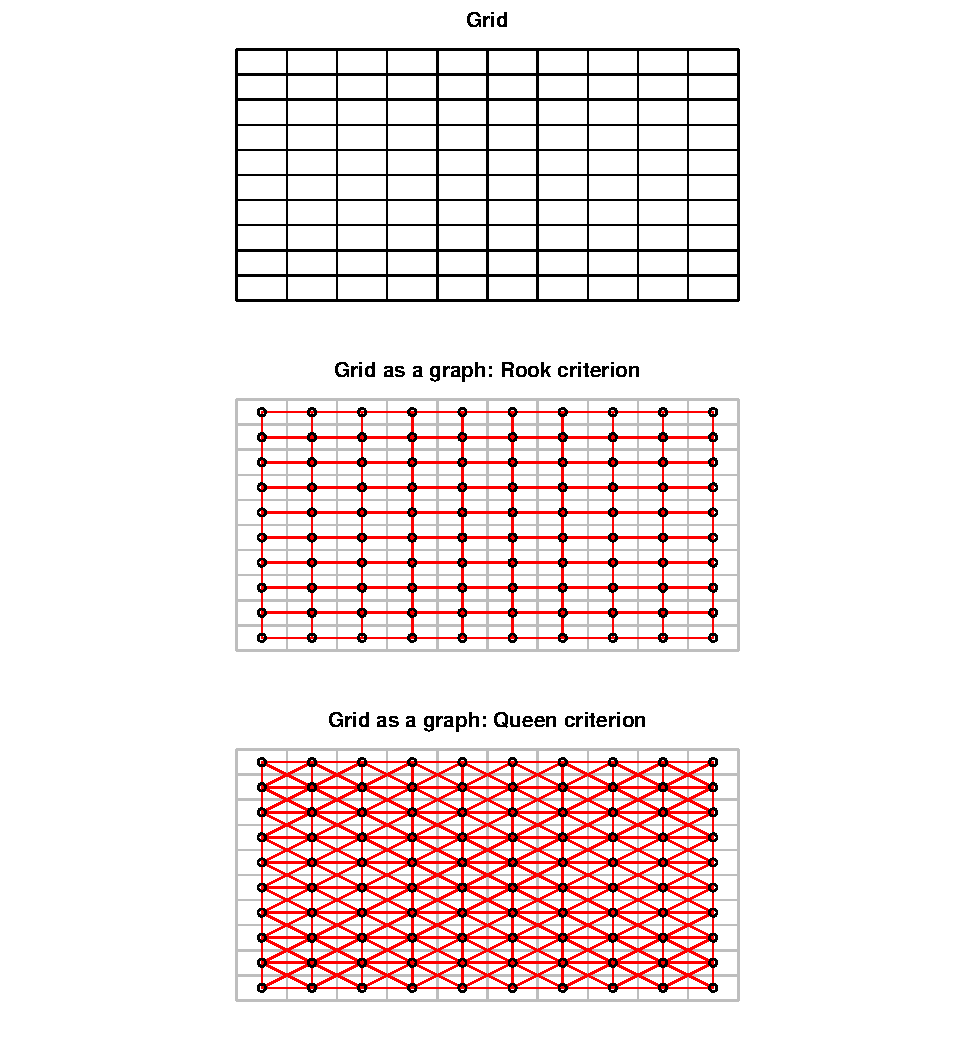
\includegraphics{Cost-Functions-for-Walking-Accessibility_files/figure-latex/figure-grid-as-graph-1.pdf}
\caption{\label{fig:figure-grid-as-graph}Converting a grid into graphs
using the Rook and Queen criteria}
\end{figure}

\hypertarget{resistancecost-as-relational-information-in-a-graph}{%
\section{3.2 Resistance/cost as relational information in a
graph}\label{resistancecost-as-relational-information-in-a-graph}}

Relational information in a graph concerns an attribute that is specific
to a node pair \(i-j\). This information can be directed, meaning that
the relation between \(i-j\) can differ from the relation between
\(j-i\). Of particular relevance for the present discussion is the fact
that links in a network can store information pertaining to transitions
between nodes. Accordingly, a key item of relational information is the
\emph{resistance} or \emph{cost} to transition between nodes in the
graph. Resistance is a property of a link that measures friction to
movement: the higher the resistance between two nodes, the more
difficult it is to transition between them.

There are different ways of defining resistance. When a DEM is
available, two physical aspects of the landscape that relate to
resistance can be obtained directly from the grid, namely the vertical
displacement and the horizontal displacement between nodes \(i\) and
\(j\). The friction to movement is greater as the vertical and/or
horizontal displacements increase (\(\Delta v\) and \(\Delta h\)
respectively). Put differently, it becomes more expensive to transition
from \(i\) to \(j\) as the distance between them in the horizontal
and/or vertical direction increases.

On a flat, homogeneous plain, the horizontal distance is a reasonable
measure of cost. Perhaps the simplest measure of resistance is the
Euclidean distance between two arbitrary (and possibly non-contiguous)
nodes \(i\) and \(k\). This distance can be calculated by means of the
Pythagorean theorem for small regions. Alternatively, for large regions,
the great circle distance can be used, to account for the curvature of
the Earth. These measures of distance do not require calculations on a
raster, only the coordinates of the two nodes. On the other hand, when
the landscape is not flat and/or is non-homogeneous, the horizontal
distance becomes suspect as a measure of resistance. In this case, we
might be interested in measuring resistance in other ways, for instance
by considering the distance on the surface, the time that it takes to
travel between nodes as a function of speed, or the energy needed to
move between the nodes.

The distance on the surface of a landscape is a somewhat more
sophisticated measure of resistance. Given a function \(y=f(x)\) that
describes a transect on the surface of a landscape, the length
\(\mathcal{L}\) of the segment of the line representing the distance on
the surface between points \(i\) and \(j\) is given by:

\begin{equation} \label{eq:1}\mathcal{L} = \int_{i}^{j}{\sqrt{1 + \frac{dy}{dx}^2}}dx\end{equation}

\noindent where \(x\) is the horizontal coordinate on the transect and
\(y\) is the elevation.

A grid is essentially a discrete representation of the landscape, and
therefore the length of the segment of a transect would instead be
calculated for \(n\) line sub-segments between locations \(i\) and \(j\)
as follows:

\begin{equation} \label{eq:2}L = \sum_{i}^{n}{d_i} = \sum_{i}^{n}{\sqrt{\Delta v_{ij}^2 + \Delta h_{ij}^2}}\end{equation}

Given vertical displacement \(\Delta v\) and the horizontal displacement
\(\Delta h\), we can approximate the distance on the surface \(L\), as
the sum of segmental distances \(d_i\). The approximation is only
limited by the resolution of the grid: higher resolutions with small
cells allow for better approximations of the distance on the surface of
the landscape.

Another feature of the landscape that can be calculated from the
vertical and horizontal displacements is the slope \(m\). The
instantaneous slope is given by the derivative of \(y = f(x)\) with
respect to \(x\). In the case of a grid, this is given by the following
expression:

\begin{equation} \label{eq:3}m = \frac{\Delta v}{\Delta h}\end{equation}

The slope is not typically used as a measure of resistance; however, it
is an intermediate attribute that is linked to speed via Tobler's
formula for hiking travel (Tobler 1993):

\begin{equation} \label{eq:4}s = 100e^{(-3.5|m + 0.05|)}\end{equation}

\noindent where the speed \(s\) is in \(m/min\). To obtain a measure of
resistance, the hiking speed in turn can be converted into travel time
in minutes if we divide the distance by speed as follows:

\begin{equation} \label{eq:5}t = \frac{d_i}{100e^{-3.5|m + 0.05|}} = \frac{1}{100}d_i \cdot e^{3.5|m + 0.05|}\end{equation}

\noindent where \(d_i\) can be the distance on the surface as discussed
above, or can be approximated by the horizontal distance \(\Delta h\)
(see Etten 2017, 13--16). Other speed formulas, including backpacker
equations, are discussed by Doherty et al. (2014) and Herzog (2010).

The slope is also linked to the energy required to move. Minetti et
al.~(2002) investigated the metabolic energy cost of human movement on
extreme slopes. This work updated and extended earlier work on the
energy cost of walking on level surfaces (e.g., Marcaria 1938; Bobbert
1960) by examining a wider range of slope and speed values. Minetti and
colleagues present an equation that relates the metabolic energy cost of
walking to slope, as follows:

\begin{equation} \label{eq:6}C_w = 280.5m^5 - 58.7m^4 - 76.8m^3 + 51.9m^2 + 19.6m + 2.5\end{equation}

\noindent where \(m\) is the slope and \(C_w\)
(\(J\cdot kg^{-1}\cdot m^{-1}\)) is the energy cost of moving one unit
of mass a horizontal distance equivalent to one unit of vertical
displacement. Notice that due to the polynomial formulation, this
equation is valid for a range of slopes approximately between \(-0.5\)
and \(0.5\), outside of which the behavior of the function becomes
counterintuitive.

Surface distance can be rewritten as a function of slope as follows:

\begin{equation} \label{eq:7}d = \sqrt{1 + m^2}\end{equation}

The three resistance functions above (Equations \ref{eq:5}, \ref{eq:6},
and \ref{eq:7}) can be expressed in similar terms. As seen in Figure
\ref{fig:figure-resistance-functions}, resistance tends to increase as
the slope increases. Surface distance and travel time are symmetric,
although travel time is shifted to the left, to reflect somewhat shorter
travel times (equivalently higher speeds) when the slope is moderately
negative (reflective of movement along a gentle downward slope). The
metabolic energy cost, in contrast, is not symmetric, and is further
shifted to the left. This is because the metabolic cost of moving up a
slope tends to be much higher than the cost of moving down a slope.

\begin{figure}
\centering
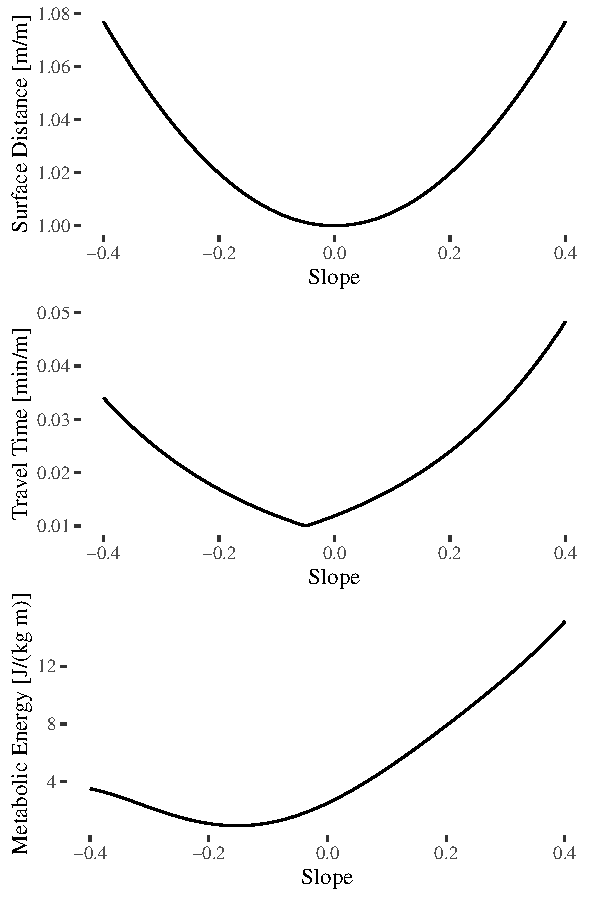
\includegraphics{Cost-Functions-for-Walking-Accessibility_files/figure-latex/figure-resistance-functions-1.pdf}
\caption{\label{fig:figure-resistance-functions}Various types of
resistance as a function of slope (plots of equations 2, 5, and 6)}
\end{figure}

\hypertarget{conductance}{%
\section{3.3 Conductance}\label{conductance}}

Resistance is an intuitive way of thinking about the way the landscape
tends to impose a cost to movement. When resistance is used it becomes
necessary to impose some constraint to avoid ``jumps'' across the
landscape, that is, non-continuous movement between cells that are not
neighbors on the grid. In practice, this entails setting the resistance
of non-contiguous pairs of nodes to a very large value (e.g., +Inf).
Computationally, this has the disadvantage of requiring dense matrices
to be stored, since every value must be explicitly retained (Etten 2017,
3). A more efficient approach involves working with the
\emph{conductance}, which is simply defined as the inverse of the
resistance. Consequently, relational information for non-contiguous
nodes can be set to zero. This allows the use of sparse matrix
techniques, whereby only non-zero values are explicitly stored and zero
values are ignored. The \texttt{gdistance} package, for example, works
internally with the conductance. This means that instead of using, e.g.,
travel time for its calculations, it uses the inverse of time (or
temporal rate), even if it reports the resistance (i.e., the time).

\hypertarget{shortest-paths-cost-and-accessibility-indicators}{%
\section{3.4 Shortest paths, cost, and accessibility
indicators}\label{shortest-paths-cost-and-accessibility-indicators}}

Given a graph and resistance/conductance information, shortest paths and
costs can be found using a conventional algorithm, such as Djikstra
(e.g., Cherkassky, Goldberg, and Radzik 1996).

Once the shortest paths have been obtained, accessibility can be
calculated based on the associated costs. A general formulation of
accessibility is as follows (see Paez, Scott, and Morency 2012):

\begin{equation} \label{eq:8}A_i = \sum_{j\in D}g(W_j)f(c_{ij})\end{equation}

\noindent where \(i\) is a point of origin and \(j\) corresponds to a
destination in the set of locations \(D\) (\(\{j \in D|j=1,\dots,J\}\)).
The functions \(g(\cdot)\) and \(f(\cdot)\) modify the opportunities
\(W\) at \(j\) and the cost \(c_{ij}\) of moving between locations \(i\)
and \(j\), respectively. In this way, accessibility \(A_i\) is a
weighted sum of opportunities, with weights that vary on the cost of
reaching \(j\) from \(i\).

Common formulations of accessibility include cumulative opportunities
with \(g(W_j)=W_j\) and \(f(c_{ij})=I(c_{ij}\le c^*)\):

\begin{equation} \label{eq:9}A_i = \sum_{j\in D}W_jI(c_{ij})\le c^*)\end{equation}

\noindent where \(I(\cdot)\) is an indicator function that takes the
value of one if the argument is true and zero otherwise, and \(c^*\) is
a cut-off or threshold value.

Gravity-type measures include inverse distance decay:

\begin{equation} \label{eq:10}A_i = \sum_{j\in D}\frac{W_j}{c_{ij}^\alpha}\end{equation}

\noindent where \(\alpha\) is a cost decay parameter, and the negative
exponential:

\begin{equation} \label{eq:11}A_i = \sum_{j\in D}W_jexp\Big(-\alpha \frac{c_{ij}}{c^*}\Big)\end{equation}

\noindent where \(c^*/\alpha\) is a kernel bandwidth that controls the
rate of cost decay.

\hypertarget{empirical-example}{%
\section{4 Empirical example}\label{empirical-example}}

In this section we apply the methods discussed in the preceding sections
to an empirical case study. Note that the source file for this paper is
a reproducible R markdown document which, along with the data files, can
be obtained from the following repository:

https://github.com/paezha/Cost-Functions-for-Walking-Accessibility

\hypertarget{context-accessibility-to-water}{%
\section{4.1 Context: accessibility to
water}\label{context-accessibility-to-water}}

In 2010, the right to safe drinking water was recognized by the United
Nations (2010) in resolution A/RES/64/292. Globally, 785 million people
still do not have access to basic drinking water services, defined as an
improved source that takes less than 30 minutes round trip, including
queuing time (UNICEF-WHO 2019). By 2030, the world has committed to
ensuring universal access to safely managed water supplies, i.e.,
sufficient supplies located on the premises and free from contamination
(UNICEF-WHO 2019). In order to meet this Sustainable Development Goal
(SDG) target (6.1), representative measures of accessibility will be
critical for the determination of equitable water point locations. Note
that 30 minutes is not how much individuals are willing or even able to
travel, but rather a threshold for how much (at most) they should
travel. In this sense, accessibility is a normative indicator (see Paez,
Scott, and Morency 2012).

\hypertarget{case-study}{%
\section{4.2 Case study}\label{case-study}}

The case study is based on a Maasai-operated group ranch in Kenya. The
members of this group ranch have settled seven neighborhoods on the
outskirts of the land managed by the group. Field-based research with
members of these communities revealed that inadequate access to drinking
water was a priority area of concern. As result of this research, a
mixed-methods collaborative study was launched to better understand the
situation and to support decision-making (Barber et al. 2018).

As part of the study, GPS coordinates were collected for homesteads
(called \emph{bomas}) and water points in three of the neighborhoods in
the group ranch. For analysis, the geospatial information is combined
with a DEM to empirically explore the implications of using different
cost functions (i.e., straight line distance, surface distance, travel
time, and metabolic energy) in the analysis of accessibility to water
points. Ultimately, this has implications for water point locations and
equity.

Raster data (DEM) were obtained from Japan Aerospace Exploration Agency
(JAXA) (https://www.eorc.jaxa.jp/ALOS/en/aw3d30/data/index.htm). The
spacing of the raster is 1 arcsec (approximately 30 m) and elevation
values are average over the range of 1 arcsec grid pixel rounded to the
integer. To protect the privacy of respondents, all coordinates in this
study are set to a false origin. As seen in Figure
\ref{fig:figure-study-area}, the study area is approximately 8.1 km in
the east-west direction, and 10 km in the north-south direction. The
maximum difference in elevation is approximately 340 m. The locations of
water sources are shown as red triangles, and bomas surveyed appear as
white crosses.

\begin{figure}
\centering
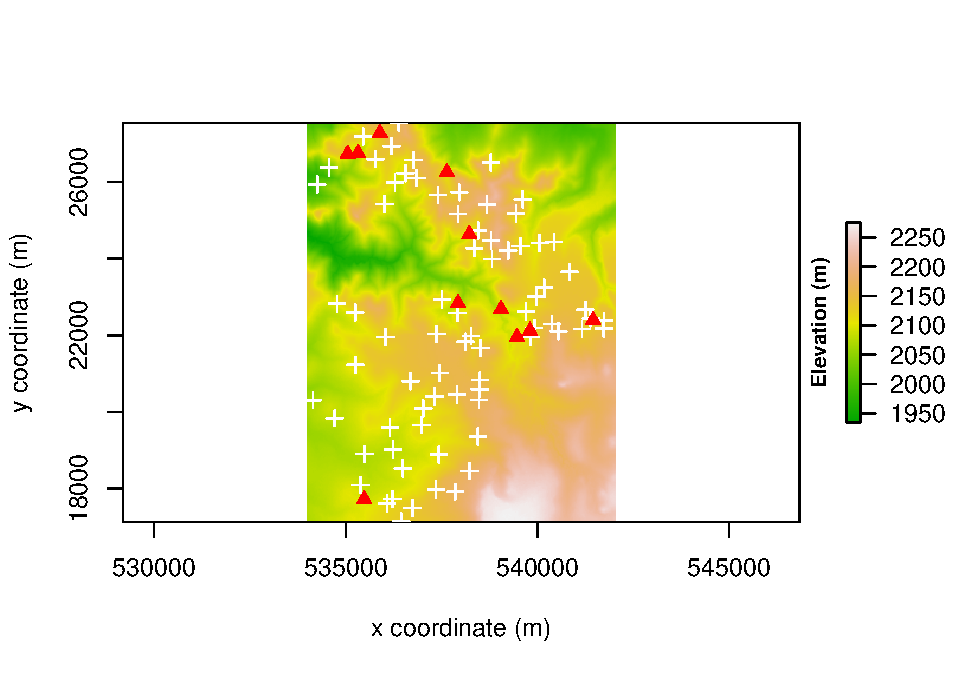
\includegraphics{Cost-Functions-for-Walking-Accessibility_files/figure-latex/figure-study-area-1.pdf}
\caption{\label{fig:figure-study-area}Digital elevation model and
location of water sources (red triangles) and bomas (white crosses) in a
region in Kenya (false origin)}
\end{figure}

\hypertarget{shortest-path-analysis}{%
\section{4.3 Shortest path analysis}\label{shortest-path-analysis}}

There are several studies in the literature that report differences in
paths when the definition of resistance changes (see inter alia Wood and
Wood 2006, Fig.1; Herzog 2010, Fig. 3; Schamel and Job 2017, Fig. 3;
Fonte, Parcero-Oubina, and Costa-Garcia 2017, Fig. 12; Kunitz, Lagree,
and Weinig 2017, Fig. 8). However, to the best of our knowledge, there
are no systematic investigations of these differences. Do least-distance
paths generally coincide with least-time paths? How often do
least-energy paths diverge from the other two? To answer these questions
in our empirical example, we begin by calculating the shortest paths.
Shortest path calculations are implemented using the centroids of all
raster cells in the study region as origins, and the water points as
destinations. Calculations are based on straight-line distance, and
functions for surface distance, time, and metabolic energy. Time and
metabolic energy include the return-trip.

Figure \ref{fig:figure-shortest-paths-kenya} shows examples of shortest
paths on the digital elevation model, according to different cost
criteria. These examples show that the paths obtained using surface
distance and time (i.e., least-distance and least-time) produce very
similar results. As noted above (Figure
\ref{fig:figure-resistance-functions}), surface distance and speed
change with slope in similar ways: both functions are symmetric on
either side of their global minima, and the hiking function is only
slightly shifted to the left, but perhaps not enough to make a practical
difference in most situations. In contrast, when the criterion for
resistance is metabolic energy (i.e., least-energy), the shortest paths
are quite different. The function for metabolic energy is distinct from
the surface distance and hiking speed functions in two important
respects: it is not symmetric, and its minimum in the interval of
interest is shifted to the left further than the hiking speed function.
This reflects a more marked preference to reduce upward movement on
slopes as the examples make clear; for instance, the outward trip may be
more advantageous if following a route that presents more moderate
downward slopes, whereas the return trip may try to avoid slopes as much
as possible. This accounts for the change in routes depending on
direction. Additionally, as seen in the figure, this function results in
the kind of zig-zagging behavior often observed in movement on sloped
terrain (Llobera and Sluckin 2007).

More generally, paths when minimizing surface distance are not perfectly
symmetric in the outward and return trips, although the differences tend
to be minimal. Symmetry is increasingly lost when minimizing time. As
suggested by the scatterplots in Figure
\ref{fig:figure-scatterplots-kenya}, the minimum surface distance and
minimum time paths diverge more in real terrain - although they are
still more direct routes between origins and destinations compared to
the minimum metabolic energy paths. Minimizing metabolic energy results
in paths that are substantially different from those estimated
minimizing travel time and distance, and also less symmetric across the
to and from directions.

Summary statistics of the costs associated with all shortest paths in
this example are shown in Table
\ref{tab:table-empirical-example-results}. The summary statistics are
obtained after calculating the shortest path from the centroids of all
raster cells to all water sources. It can be seen there that the
correlation between Euclidean and surface distance is practically
perfect. The correlations between Euclidean distance and time, on the
one hand, and energy, on the other, are weaker. Energy correlates only
moderately with surface distance and travel time, and in these two cases
it does so with a great deal of dispersion, especially for longer trips
(see Figure \ref{fig:figure-scatterplots-kenya}). These results indicate
that while straight line distance and surface distance might be
reasonably used interchangeably, the same is not necessarily true of
other measures of cost, particularly metabolic energy.

\begin{table}

\caption{\label{tab:table-empirical-example-results}\label{tab:table-empirical-example-results}Summary statistics of the cost of shortest paths according to different definitons of cost in the empirical example}
\centering
\resizebox{\linewidth}{!}{
\begin{tabular}[t]{lrrrrrrrrrr}
\toprule
\multicolumn{1}{c}{ } & \multicolumn{6}{c}{Summary Statistics} & \multicolumn{4}{c}{Correlation} \\
\cmidrule(l{3pt}r{3pt}){2-7} \cmidrule(l{3pt}r{3pt}){8-11}
Resistance & Min. & X1st.Qu. & Median & Mean & X3rd.Qu. & Max. & Euclidean & Surface & Time & Energy\\
\midrule
Euclidean Distance & 2.43 & 2983.68 & 4530.69 & 4754.05 & 6282.97 & 11860.49 & 1.00 & 1.00 & 0.67 & 0.49\\
Surface Distance & 0.00 & 3153.71 & 4787.95 & 5025.20 & 6624.31 & 12711.88 & 1.00 & 1.00 & 0.67 & 0.49\\
Travel Time & 5.36 & 99.76 & 129.38 & 130.57 & 160.01 & 288.82 & 0.67 & 0.67 & 1.00 & 0.78\\
Metabolic Energy & 806.91 & 29973.08 & 41599.21 & 41337.54 & 51851.57 & 105921.65 & 0.49 & 0.49 & 0.78 & 1.00\\
\bottomrule
\multicolumn{11}{l}{\textit{Note: }}\\
\multicolumn{11}{l}{Euclidean and Surface distances are in m; Time is in min; Metabolic energy is in J (baseline weight is 50 kg)}\\
\end{tabular}}
\end{table}

\begin{figure}
\centering
\includegraphics{Cost-Functions-for-Walking-Accessibility_files/figure-latex/figure-scatterplots-kenya-1.pdf}
\caption{\label{fig:figure-scatterplots-kenya}Scatterplots of shortest
path costs for different definitions of resistance: empirical example}
\end{figure}

\begin{figure}
\centering
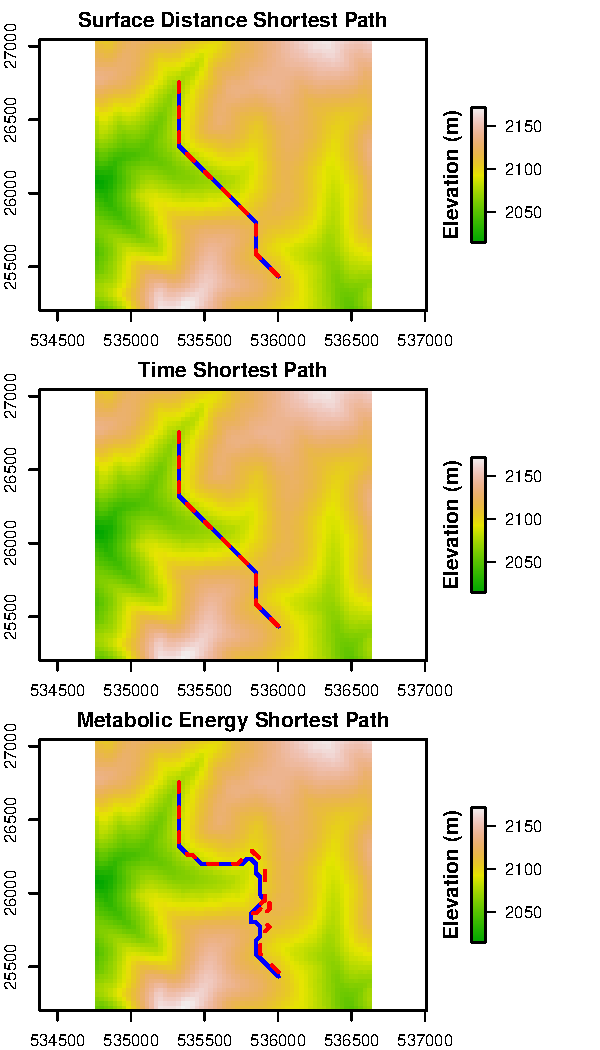
\includegraphics{Cost-Functions-for-Walking-Accessibility_files/figure-latex/figure-shortest-paths-kenya-1.pdf}
\caption{\label{fig:figure-shortest-paths-kenya}Examples of shortest
paths using different definitions of resistance, case study (blue path
is origin-destination, red dashed path is destination-origin, i.e.,
return trip)}
\end{figure}

Inspection of the summary statistics raises a relevant question: how
much do costs diverge when paths based on different criteria are used?
Consider the paths shown in Figure
\ref{fig:figure-shortest-paths-kenya}. For the same origin-destination
pair, there is a minimum surface-distance path, a minimum time path, and
a minimum metabolic energy path. These are all generally different from
each other. However, what is the surface distance over the minimum time
path? And how different is it from the surface distance when it was
minimized? Similarly, it is evident that minimum metabolic energy paths
are longer than minimum surface distance and time paths, but by how
much? To explore these questions, we take the origins and destinations
in the empirical example (i.e., \(73\) bomas and \(11\) water points)
and calculate the shortest paths according to surface distance, time,
and energy criteria. Then, we re-analyze each shortest path to calculate
the equivalent surface distance, equivalent time, and equivalent energy.
The results of this analysis are shown in Figure
\ref{fig:figure-scatterplots-equivalent-cost-kenya}.

In the scatterplots, the \(x\)-axis is the cost that was minimized. In
the \(y\)-axis is the equivalent cost for the path between the same
origin-destination pair. The black line is the \(45\)-degree (i.e., the
identity) line. Notice that the equivalent cost is \emph{at least} the
same as the minimized cost. This happens when the costs for the two
criteria are identical for a path. More generally, the equivalent cost
tends to be higher. That said, the surface distance over minimum time
paths tends to be very similar to the minimum surface distance. The
similarity is less marked in the converse case: times over minimum
surface distance paths tend to be markedly longer than minimum times.
The most important divergences are in terms of metabolic energy.
Equivalent surface distance and time are considerably longer over
minimum energy paths. Likewise, equivalent energy tends to be
considerably higher over minimum surface distance and time paths.

These results indicate, again, that surface distance and time are
potentially good proxies for each other, but neither is a good proxy for
metabolic energy. In the following section this is seen more clearly
when the results of the shortest path analysis are used for creating
accessibility surfaces.

\begin{figure}
\centering
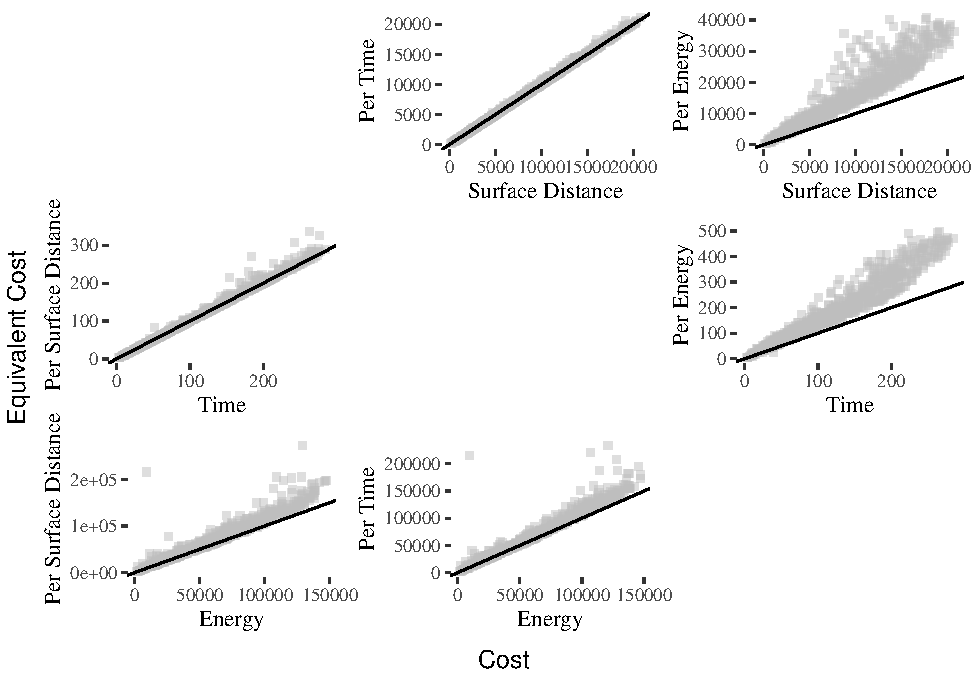
\includegraphics{Cost-Functions-for-Walking-Accessibility_files/figure-latex/figure-scatterplots-equivalent-cost-kenya-1.pdf}
\caption{\label{fig:figure-scatterplots-equivalent-cost-kenya}Scatterplots
of shortest path costs and equivalent cost for different definitions of
resistance}
\end{figure}

\hypertarget{accessibility-analysis}{%
\section{4.4 Accessibility analysis}\label{accessibility-analysis}}

Once the shortest paths have been calculated, the results can be used to
implement an accessibility indicator. For this analysis we select a
cumulative opportunities measure (Equation \ref{eq:9}). The critical
value \(c^*\) for the two distance-based indicators (Euclidean and
surface) is set to \(1\) km. The critical value \(c^*\) for travel time
is \(30\) minutes for the round-trip journey (assuming that the queuing
time at the source is zero, which is not necessarily true). There are no
guidelines for how much \emph{energy} should be spent fetching water.
For the analysis we tune the critical value \(c^*\) in such a way that
the equivalent energy is similar to a round trip of \(30\) minutes.
Accessibility maps are shown in Figure
\ref{fig:figure-accessibility-cumulative-opportunities-kenya}.

The levels of accessibility are counts of accessible opportunities. As
such, some regions have accessibility to zero water points, or to one
water point, two water points, and so on. Bearing this in mind, the red
regions indicate high priority areas for intervention since they do not
satisfy the criteria for basic service, i.e., accessibility to at least
one water source. Accessibility based on straight-line distance leads
(as expected) to circular service areas. This symmetry is lost
progressively as the effects of the landscape are captured by other cost
functions. Still, surface distance and travel time are remarkably
similar, although travel time, even accounting for the return trip,
gives a slightly more generous picture of accessibility than the
distance criteria. In line with the discussion in the preceding
subsection, metabolic energy-based accessibility is distinct, and does
not replicate the somewhat artificial circular catchment areas around
water sources. According to this criterion (keeping in mind that it was
tuned to match a \(30\)-minute travel time) there are fewer regions that
lack basic access in the study area.

\begin{figure}
\centering
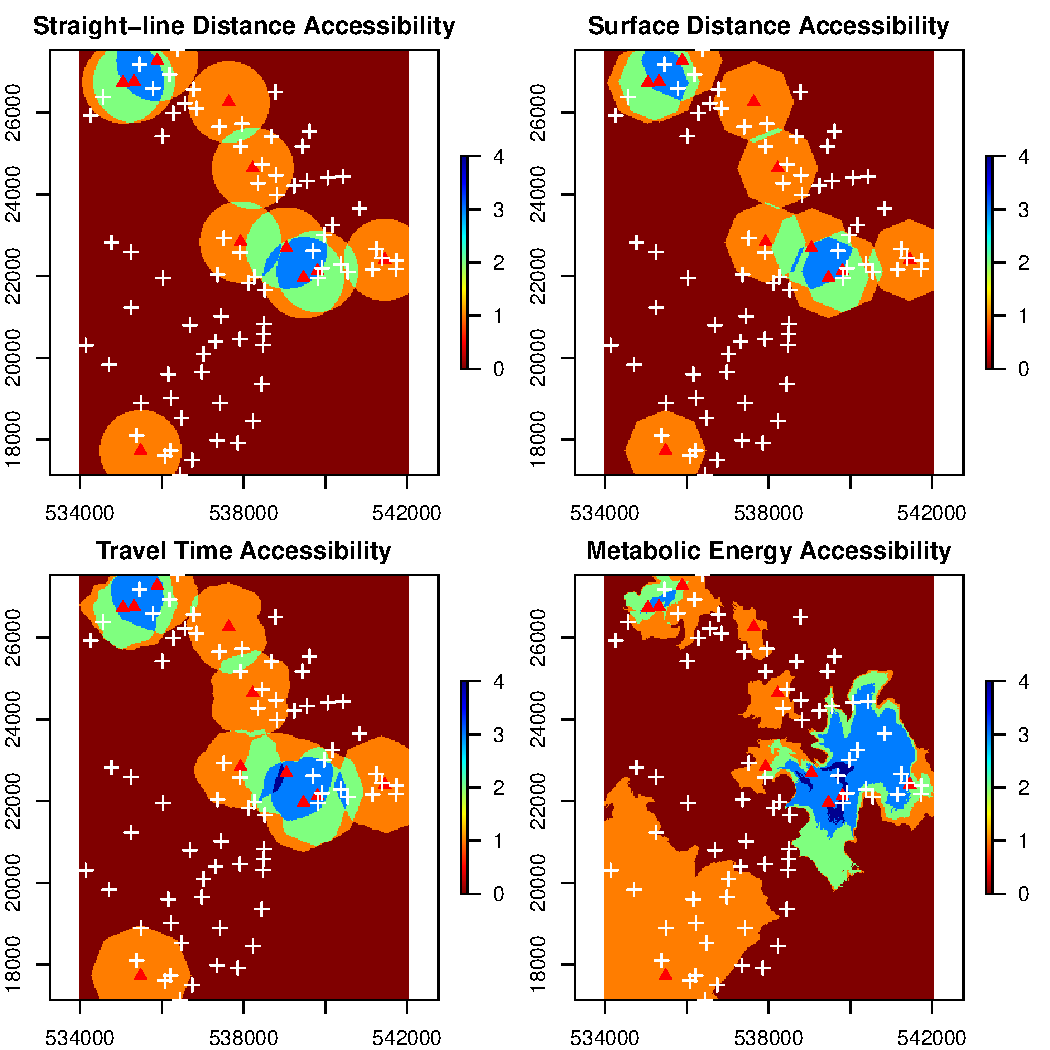
\includegraphics{Cost-Functions-for-Walking-Accessibility_files/figure-latex/figure-accessibility-cumulative-opportunities-kenya-1.pdf}
\caption{\label{fig:figure-accessibility-cumulative-opportunities-kenya}Cumulative
opportunities accessibility maps in empirical example using different
measures of resistance (Red = 0 water sources; Orange = 1 water source;
Green = 2 water sources; Light Blue = 3 water sources; Dark Blue = 4
water sources)}
\end{figure}

\begin{table}

\caption{\label{tab:table-summary-accessibility}\label{tab:table-summary-accessibility}Summary of accessibility analysis in case study: number of bomas with different levels of accessibility to water sources by cost criteria}
\centering
\begin{tabular}[t]{lcccc}
\toprule
\multicolumn{1}{c}{} & \multicolumn{4}{c}{Cost Criterion} \\
\cmidrule(l{3pt}r{3pt}){2-5}
Water Sources & Euclidean Distance & Surface Distance & Time & Energy\\
\midrule
0 & 41 & 42 & 38 & 40\\
1 & 22 & 24 & 24 & 17\\
2 & 7 & 4 & 5 & 5\\
3 & 3 & 3 & 6 & 8\\
4 & 0 & 0 & 0 & 3\\
\bottomrule
\end{tabular}
\end{table}

Table \ref{tab:table-summary-accessibility} presents the summary of
results of the accessibility analysis from the perspective of bomas. The
number of bomas with zero accessibility are 41 according to straight
line distance, 42 according to surface distance, 41 according to
straight line distance, 38 according to travel time, and 41 according to
straight line distance, 40 according to metabolic energy. More bomas
appear to have greater accessibility to water according to travel time
and metabolic energy than either distance criteria.

\hypertarget{discussion}{%
\section{4.5 Discussion}\label{discussion}}

The empirical example illustrates how there are potentially important
differences in the conclusions that would be drawn depending on which
cost criterion is used in the implementation of accessibility analysis.
This prompts the question: what do we measure when we measure
accessibility? An implicit (and often under-examined) assumption in many
treatments of accessibility concerns the kind of behavior that
accessibility analysis is meant to reflect (Paez, Scott, and Morency
2012). As the analysis above illustrates, this might not be critical
when Euclidean distance, surface distance, and travel time are used,
given the similarities in outcomes between least-distance and least-time
behaviors. However, when least-effort is the determining factor, the
results may change substantially. This, in turn, can be expected to have
an impact on policy analysis and decision-making.

So, which criterion is more appropriate? The answer at this point is, we
do not know for sure. Minimization of travel time may be a suitable
assumption for some activities - for instance, when evacuating or
fleeing danger. However, the physical exertion involved in active travel
may be better represented by cost in metabolic energy - which, as our
research demonstrates, leads to results that are markedly different from
distance and time, the two most widely used criteria. In fact, assuming
that travelers minimize distance or time may lead to travel predictions
that are wholly unreflective of actual cost-minimization behavior.
Another reason this may be important is sensitivity to changes in the
assumptions. For example, the friction of distance is symmetric on the
outward and return trips. This may not be the case for travel time and
energy. Suppose for instance that speed is reduced on the return trip -
perhaps due to an increase in the load, if, for example, the purpose of
the trip is to fetch water. Likewise, the metabolic energy requirements
would increase with the load. In an infrastructure-poor context, our
results show that longer, more time-consuming paths may be taken in
exchange for reduced energy consumption. Such a scenario may be a valid
hypothesis for water fetching in low- and middle-income countries, if
for example, an individual fetching water is more concerned with
metabolic pressures than time pressures. As a result, they may trade off
distance and time for reduced energy expenditure in the to and from
directions. Water fetching in sub-Saharan Africa broadly, and Kenya
specifically, is a gendered norm that falls on women and girls and is
exacerbated by pregnancy (women's reproductive role in society; Moser
1993). Given the existence of multi-directional relationships between
nutritional requirements, time and energy required for water fetching,
and susceptibility towards domestic violence if daily household duties
are not completed (Pommells et al. 2018), metabolic energy may be a more
important, if subconscious, choice factor in determining a
water-fetching path.

This is not to say that an emphasis on minimizing travel time for
reaching water by entities such as the World Health Organization is
misplaced, only that its use should be more explicitly recognized and
critically examined relative to assumptions about different travel
behavior and mobility contexts. When an individual is travelling via a
motorized mode, such as driving a car or riding transit, the
minimization of travel time or distance seems like a reasonable
assumption - the commuter with daily time constraints on available
activities within in their potential path area may indeed seek to
minimize travel time to better participate in activities of value.
Similarly, a firefighter may not prioritize energy expenditure over
travel time or distance when escaping a wildfire (Campbell, Dennison,
and Butler 2017). For active travelers who face stricter capability
constraints, for example due to nutrition deficiencies, poor health,
age, or disabilities, minimizing the metabolic energy cost might well be
a more accurate assumption about their behavior.

\hypertarget{conclusions}{%
\section{5 Conclusions}\label{conclusions}}

Research into accessibility makes some implicit assumptions about the
travel behavior of individuals that are not always recognized. Much of
the literature on accessibility specifies distance or travel time as the
primary costs to be optimized and is generally carried on in what can be
described as infrastructure-rich regions. Moreover, most research is
conducted under an assumption of topographical or topological planarity.
However, the greater availability of enhanced geographic data on the
relief of terrain, as well as advances in research into the temporal and
metabolic costs of travel enable a greater understanding of the link
between different travel cost attributes and how individuals interact
with the natural and built environments in varied contexts.

In this paper, we utilized an empirical case study in rural Kenya to
estimate the cost of active travel in an infrastructure-poor region.
This is an example of an environment rich in topography but lacking in
transportation infrastructure. Comparisons between distance, travel
time, and energy expenditure revealed interesting differences in
predicted travel paths. Results show that calculations of shortest-paths
using Euclidean distance, distance on the 3D surface, and slope-aware
travel time predicted by Tobler's Hiking Function were remarkably
similar. Paths are also virtually identical in the to and from
directions, with a predicted trajectory that is largely straight over
the surface. In retrospect, the lack of difference between the 3D
distance and travel time calculations is unsurprising, as slope and
travel time are acutely linked in the specification of Tobler's
function, particularly at more gentle path gradients. It may be that
trips with steeper gradients or over longer distances are more sensitive
to the velocity gradients in Tobler's function. When metabolic energy is
used as a measure of cost, however, strikingly different results are
found.

Our results, in the context of infrastructure-poor regions, offer
provocative implications for accessibility research more generally. At a
high level, our work challenges an implicit bias in accessibility
research towards the minimization of travel time or distance. This bias
could be understood as an outcome of early accessibility research
associated with large transportation projects, mostly for motorized
travel, in high income, infrastructure-rich countries. In this context,
the benefits were often framed in terms of travel time savings,
particularly for cost-benefit analysis. It is not difficult to imagine
travel scenarios in these regions where optimization of travel time may
not be the primary concern. For example, elderly individuals engaged in
active travel may behave in a way that minimizes energy expenditure over
time, selecting paths that offer lower metabolic resistance and reduced
risk of travel difficulty. Cyclists may also optimize route choices
based on terrain, preferring network paths that are longer but minimize
uphill travel. In this light, route choice algorithms implemented in
consumer mobile mapping software that recommend travel choices that
minimize travel time may be insensitive to the actual cost optimization
behavior of their users given different mobility and environmental
contexts. Although accessibility research continues to evolve, it may be
that these beginnings have led to a path dependency with respect to the
focus of the analytical lens on travel time and distance.

In terms of future research, it is important to note that Tobler's
hiking function and the metabolic cost function were calibrated for
particular demographic groups. In this respect, Looney et al. (2018)
discuss the need to (re)calibrate the metabolic energy functions for
special population segments (also see Looney et al. 2019, and
@Richmond2019terrain). This appears as an important direction for future
research. Metabolic energy in particular provides an intriguing avenue
for researching the cost of movement, one that makes it possible to
better understand vulnerable populations, such as older adults in urban
settings, or pregnant women in rural areas who require greater
nutritional intake and expend more energy per unit activity. Directions
for further research include certain trade-offs between route choice
variables across various applications, for example, walking and cycling
route choice algorithms.

Furthermore, it is possible to envision scenarios where travel choices
are made while optimizing several attributes simultaneously, such as the
minimization of travel time, distance, monetary cost, and/or energy
expenditure, as well as the potential for maximizing other attributes
like safety or interest. In these cases, better insight into the choices
made by individuals relative to their activities and time and mobility
constraints is required. Similarly, alternative route choice algorithms
that optimize several functions would be required to exploit this
information for improved predictive modelling of active travel choices
and accessibility. Finally, cognition imposes its own travel costs.
Erath et al. (2017), for example, include a factor to modify
\emph{actual} travel time to obtain \emph{perceived} travel time. In
addition, there might be additional time and mental costs involved in
the selection of paths on familiar or unfamiliar terrain. Cognition is
incorporated into an individual's estimation of travel times on the cost
surface through the search algorithm, and could be incorporated in
shortest paths algorithms by allowing searches to happen on higher order
spatial lags, beyond adjacent cells.

Finally, the discussion in this paper focused on the topographical
features of terrain. It would also be interesting to examine the impact
on accessibility of different land cover types, including the presence
of potential barriers that must be crossed or circumvented (e.g.,
wetlands), or facilitators to travel (e.g., dirt trails or tracks on the
terrain). This is a matter for future research.

\hypertarget{acknowledgments}{%
\section{Acknowledgments}\label{acknowledgments}}

The following \texttt{R} packages were used in the course of this
investigation and the authors wish to acknowledge their developers:
\texttt{knitr} (Xie 2015, 2018), \texttt{tidyverse} (Wickham 2017),
\texttt{raster} (Hijmans 2018), \texttt{gdistance} (Etten 2017),
\texttt{gridExtra} (Auguie 2017), \texttt{spdep} (Bivand, Pebesma, and
Gómez-Rubio 2013), \texttt{kableExtra} (Zhu 2018), \texttt{ggthemes}
(Arnold 2018), \texttt{plot3D} (Soetaert 2017), and \texttt{rticles}
(Allaire et al. 2018).

\hypertarget{references}{%
\section*{References}\label{references}}
\addcontentsline{toc}{section}{References}

\hypertarget{refs}{}
\leavevmode\hypertarget{ref-Adriaensen2003}{}%
Adriaensen, F., J. P. Chardon, G. De Blust, E. Swinnen, S. Villalba, H.
Gulinck, and E. Matthysen. 2003. ``The Application of `Least-Cost'
Modelling as a Functional Landscape Model.'' Journal Article.
\emph{Landscape and Urban Planning} 64 (4): 233--47.
\url{https://doi.org/10.1016/s0169-2046(02)00242-6}.

\leavevmode\hypertarget{ref-Alegana2012}{}%
Alegana, V. A., J. A. Wright, U. Pentrina, A. M. Noor, R. W. Snow, and
P. M. Atkinson. 2012. ``Spatial Modelling of Healthcare Utilisation for
Treatment of Fever in Namibia.'' Journal Article. \emph{International
Journal of Health Geographics} 11 (6): 1--13.
\url{https://doi.org/10.1186/1476-072x-11-6}.

\leavevmode\hypertarget{ref-Allaire2018rticles}{}%
Allaire, JJ, Yihui Xie, R Foundation, Hadley Wickham, Journal of
Statistical Software, Ramnath Vaidyanathan, Association for Computing
Machinery, et al. 2018. \emph{Rticles: Article Formats for R Markdown}.
\url{https://CRAN.R-project.org/package=rticles}.

\leavevmode\hypertarget{ref-Aoun2015}{}%
Aoun, N., H. Matsuda, and M. Sekiyama. 2015. ``Geographical
Accessibility to Healthcare and Malnutrition in Rwanda.'' Journal
Article. \emph{Social Science \& Medicine} 130: 135--45.
\url{https://doi.org/10.1016/j.socscimed.2015.02.004}.

\leavevmode\hypertarget{ref-Apparicio2008}{}%
Apparicio, Philippe, Mohamed Abdelmajid, Mylène Riva, and Richard
Shearmur. 2008. ``Comparing Alternative Approaches to Measuring the
Geographical Accessibility of Urban Health Services: Distance Types and
Aggregation-Error Issues.'' \emph{International Journal of Health
Geographics} 7 (1): 7.

\leavevmode\hypertarget{ref-Arnold2018}{}%
Arnold, Jeffrey B. 2018. \emph{Ggthemes: Extra Themes, Scales and Geoms
for 'Ggplot2'}. \url{https://CRAN.R-project.org/package=ggthemes}.

\leavevmode\hypertarget{ref-Arranz2019measuring}{}%
Arranz-López, Aldo, Julio A. Soria-Lara, Frank Witlox, and Antonio Páez.
2019. ``Measuring Relative Non-Motorized Accessibility to Retail
Activities.'' Journal Article. \emph{International Journal of
Sustainable Transportation} 13 (9): 639--51.
\url{https://doi.org/10.1080/15568318.2018.1498563}.

\leavevmode\hypertarget{ref-assembly2010human}{}%
Assembly, General. 2010. ``The Human Right to Water and Sanitation
(a/Res/64/292).'' \emph{United Nations (28 July)}.

\leavevmode\hypertarget{ref-Auguie2017}{}%
Auguie, Baptiste. 2017. \emph{GridExtra: Miscellaneous Functions for
"Grid" Graphics}. \url{https://CRAN.R-project.org/package=gridExtra}.

\leavevmode\hypertarget{ref-Barber2018designing}{}%
Barber, Hilary, Sarah E Dickson-Anderson, Corinne J Schuster-Wallace,
Susan J Elliott, and Saaya Tema. 2018. ``Designing a Mixed-Methods
Approach for Collaborative Local Water Security: Findings from a Kenyan
Case Study.'' \emph{Exposure and Health}, 1--9.

\leavevmode\hypertarget{ref-Basu2014value}{}%
Basu, Debasis, and John Douglas Hunt. 2014. ``Value of Travel Time for
Home-Based School Tours in California.'' \emph{Transportation Planning
and Technology} 37 (3): 287--306.

\leavevmode\hypertarget{ref-Bivand2013asdar}{}%
Bivand, R. S., E. J. Pebesma, and V. Gómez-Rubio. 2013. \emph{Applied
Spatial Data Analysis with R}. Book. Second Edition. New York: Springer
Science+Business Media. \url{http://www.asdar-book.org/}.

\leavevmode\hypertarget{ref-Bobbert1960energy}{}%
Bobbert, AC. 1960. ``Energy Expenditure in Level and Grade Walking.''
\emph{Journal of Applied Physiology} 15 (6): 1015--21.

\leavevmode\hypertarget{ref-Bocarejo2012}{}%
Bocarejo, S. J. P., and H. D. R. Oviedo. 2012. ``Transport Accessibility
and Social Inequities: A Tool for Identification of Mobility Needs and
Evaluation of Transport Investments.'' Journal Article. \emph{Journal of
Transport Geography} 24: 142--54.
\url{https://doi.org/10.1016/j.jtrangeo.2011.12.004}.

\leavevmode\hypertarget{ref-Campbell2017}{}%
Campbell, Michael J, Philip E Dennison, and Bret W Butler. 2017. ``A
Lidar-Based Analysis of the Effects of Slope, Vegetation Density, and
Ground Surface Roughness on Travel Rates for Wildland Firefighter Escape
Route Mapping.'' \emph{International Journal of Wildland Fire} 26 (10):
884--95.

\leavevmode\hypertarget{ref-Chen2017}{}%
Chen, Y. N., M. M. Schmitz, F. Serbanescu, M. M. Dynes, G. Maro, and M.
R. Kramer. 2017. ``Geographic Access Modeling of Emergency Obstetric and
Neonatal Care in Kigoma Region, Tanzania: Transportation Schemes and
Programmatic Implications.'' Journal Article. \emph{Global
Health-Science and Practice} 5 (3): 430--45.
\url{https://doi.org/10.9745/ghsp-d-17-00110}.

\leavevmode\hypertarget{ref-Cherkassky1996}{}%
Cherkassky, B. V., A. V. Goldberg, and T. Radzik. 1996. ``Shortest Paths
Algorithms: Theory and Experimental Evaluation.'' Journal Article.
\emph{Mathematical Programming} 73 (2): 129--74.
\url{https://doi.org/10.1007/bf02592101}.

\leavevmode\hypertarget{ref-Dangisso2015}{}%
Dangisso, M. H., D. G. Datiko, and B. Lindtjorn. 2015. ``Accessibility
to Tuberculosis Control Services and Tuberculosis Programme Performance
in Southern Ethiopia.'' Journal Article. \emph{Global Health Action} 8:
10. \url{https://doi.org/10.3402/gha.v8.29443}.

\leavevmode\hypertarget{ref-Doherty2014analysis}{}%
Doherty, P. J., Q. H. Guo, J. Doke, and D. Ferguson. 2014. ``An Analysis
of Probability of Area Techniques for Missing Persons in Yosemite
National Park.'' Journal Article. \emph{Applied Geography} 47: 99--110.
\url{https://doi.org/10.1016/j.apgeog.2013.11.001}.

\leavevmode\hypertarget{ref-Ebener2005}{}%
Ebener, Steeve, Zine El Morjani, Nicolas Ray, and Michael Black. 2005.
``Physical Accessibility to Health Care: From Isotropy to Anisotropy.''
Journal Article 9 (6).

\leavevmode\hypertarget{ref-Erath2017pedestrian}{}%
Erath, Alexander, Michael AB van Eggermond, Sergio A Ordóñez, and Kay W
Axhausen. 2017. ``Introducing the Pedestrian Accessibility Tool:
Walkability Analysis for a Geographic Information System.'' Journal
Article. \emph{Transportation Research Record} 2661 (1): 51--61.

\leavevmode\hypertarget{ref-ESRI2016path}{}%
ESRI. 2016. ``How the Path Distance Tools Work (Arcmap 10.3).'' Web
Page.
\url{http://desktop.arcgis.com/en/arcmap/10.3/tools/spatial-analyst-toolbox/how-the-path-distance-tools-work.htm}.

\leavevmode\hypertarget{ref-vanEtten2017}{}%
Etten, J. van. 2017. ``R Package Gdistance: Distances and Routes on
Geographical Grids.'' Journal Article. \emph{Journal of Statistical
Software} 76 (13): 1--21. \url{https://doi.org/10.18637/jss.v076.i13}.

\leavevmode\hypertarget{ref-Fonte2017}{}%
Fonte, J., C. Parcero-Oubina, and J. M. Costa-Garcia. 2017. ``A
Gis-Based Analysis of the Rationale Behind Roman Roads. THE Case of the
so-Called via Xvii (Nw Iberian Peninsula).'' Journal Article.
\emph{Mediterranean Archaeology \& Archaeometry} 17 (3): 163--89.
\url{https://doi.org/10.5281/zenodo.1005562}.

\leavevmode\hypertarget{ref-Geere2018water}{}%
Geere, J. A. L., M. Cortobius, J. H. Geere, C. C. Hammer, and P. R.
Hunter. 2018. ``Is Water Carriage Associated with the Water Carrier's
Health? A Systematic Review of Quantitative and Qualitative Evidence.''
Journal Article. \emph{Bmj Global Health} 3 (3): 24.
\url{https://doi.org/10.1136/bmjgh-2018-000764}.

\leavevmode\hypertarget{ref-Geurs2009}{}%
Geurs, K., W. Boon, and B. Van Wee. 2009. ``Social Impacts of Transport:
Literature Review and the State of the Practice of Transport Appraisal
in the Netherlands and the United Kingdom.'' Journal Article.
\emph{Transport Reviews} 29 (1): 69--90.
\url{ISI:000261193500004\%0AC:/Papers/Transport\%20Reviews/Transport\%20Reviews\%20(2009)\%2029\%20(1)\%2069-90.pdf}.

\leavevmode\hypertarget{ref-Gutierrez2008}{}%
Gutierrez, Javier, Juan Carlos J Environment Garcia-Palomares, Planning
B: Planning, and Design. 2008. ``Distance-Measure Impacts on the
Calculation of Transport Service Areas Using Gis.'' Journal Article 35
(3): 480--503.

\leavevmode\hypertarget{ref-Gutierrez1996}{}%
Gutierrez, J., and P. Urbano. 1996. ``Accessibility in the Eu: The
Impact of Trans-European Network.'' Journal Article. \emph{Journal of
Transport Geography} 4 (1): 15--25.

\leavevmode\hypertarget{ref-Gutierrez1999impact}{}%
Gutiérrez, Javier, and Gabriel Gómez. 1999. ``The Impact of Orbital
Motorways on Intra-Metropolitan Accessibility: The Case of Madrid's
M-40.'' Journal Article. \emph{Journal of Transport Geography} 7 (1):
1--15. \url{https://doi.org/10.1016/s0966-6923(98)00029-5}.

\leavevmode\hypertarget{ref-Herzog2010theory}{}%
Herzog, Irmela. 2010. ``Theory and Practice of Cost Functions.'' In
\emph{Fusion of Cultures. Abstracts of the Xxxviii Conference on
Computer Applications and Quantitative Methods in Archaeology}, edited
by Javier Melero, Pedro Cano, and Jorge Revelles, 431--34.

\leavevmode\hypertarget{ref-Hijmans2018raster}{}%
Hijmans, Robert J. 2018. \emph{Raster: Geographic Data Analysis and
Modeling}. \url{https://CRAN.R-project.org/package=raster}.

\leavevmode\hypertarget{ref-Ho2014}{}%
Ho, J. C., K. C. Russel, and J. Davis. 2014. ``The Challenge of Global
Water Access Monitoring: Evaluating Straight-Line Distance Versus
Self-Reported Travel Time Among Rural Households in Mozambique.''
Journal Article. \emph{Journal of Water and Health} 12 (1): 173--83.
\url{https://doi.org/10.2166/wh.2013.042}.

\leavevmode\hypertarget{ref-Hou2011transport}{}%
Hou, Q., and S. M. Li. 2011. ``Transport Infrastructure Development and
Changing Spatial Accessibility in the Greater Pearl River Delta, China,
1990-2020.'' Journal Article. \emph{Journal of Transport Geography} 19
(6): 1350--60. \url{https://doi.org/10.1016/j.jtrangeo.2011.07.003}.

\leavevmode\hypertarget{ref-Hsu2014energy}{}%
Hsu, C. I., and Y. C. Tsai. 2014. ``An Energy Expenditure Approach for
Estimating Walking Distance.'' Journal Article. \emph{Environment and
Planning B-Planning \& Design} 41 (2): 289--306.
\url{https://doi.org/10.1068/b37169}.

\leavevmode\hypertarget{ref-iacono2010}{}%
Iacono, Michael, Kevin J Krizek, and Ahmed El-Geneidy. 2010. ``Measuring
Non-Motorized Accessibility: Issues, Alternatives, and Execution.''
\emph{Journal of Transport Geography} 18 (1): 133--40.

\leavevmode\hypertarget{ref-Iseki2014approach}{}%
Iseki, H., and M. Tingstrom. 2014. ``A New Approach for Bikeshed
Analysis with Consideration of Topography, Street Connectivity, and
Energy Consumption.'' Journal Article. \emph{Computers Environment and
Urban Systems} 48: 166--77.
\url{https://doi.org/10.1016/j.compenvurbsys.2014.07.008}.

\leavevmode\hypertarget{ref-Jobe2009new}{}%
Jobe, R. T., and P. S. White. 2009. ``A New Cost-Distance Model for
Human Accessibility and an Evaluation of Accessibility Bias in Permanent
Vegetation Plots in Great Smoky Mountains National Park, Usa.'' Journal
Article. \emph{Journal of Vegetation Science} 20 (6): 1099--1109.
\url{https://doi.org/10.1111/j.1654-1103.2009.01108.x}.

\leavevmode\hypertarget{ref-Kuniz2017}{}%
Kunitz, J. K., J. D. Lagree, and D. L. Weinig. 2017. ``A Gis Examination
of the Chacoan Great North Road.'' Journal Article. \emph{Kiva-Journal
of Southwestern Anthropology and History} 83 (1): 86--113.
\url{https://doi.org/10.1080/00231940.2016.1199936}.

\leavevmode\hypertarget{ref-Larouche2014}{}%
Larouche, Richard, Adewale L Oyeyemi, Antonio Prista, Vincent Onywera,
Kingsley K Akinroye, and Mark S Tremblay. 2014. ``A Systematic Review of
Active Transportation Research in Africa and the Psychometric Properties
of Measurement Tools for Children and Youth.'' \emph{International
Journal of Behavioral Nutrition and Physical Activity} 11 (1): 129.

\leavevmode\hypertarget{ref-Linneker1992accessibility}{}%
Linneker, B. J., and N. A. Spence. 1992. ``An Accessibility Analysis of
the Impact of the M25 London Orbital Motorway on Britain.'' Journal
Article. \emph{Regional Studies} 26 (1): 31--47.
\url{ISI:A1992HJ27600003}.

\leavevmode\hypertarget{ref-Llobera2007}{}%
Llobera, M., and T. J. Sluckin. 2007. ``Zigzaggining: Theoretical
Insights on Climbing Strategies.'' Journal Article. \emph{Journal of
Theoretical Biology} 249 (2): 206--17.
\url{https://doi.org/10.1016/j.jtbi.2007.07.020}.

\leavevmode\hypertarget{ref-Looney2019metabolic}{}%
Looney, D. P., A. W. Potter, J. L. Pryor, P. E. Bremner, C. R. Chalmers,
H. L. McClung, A. P. Welles, and W. R. Santee. 2019. ``Metabolic Costs
of Standing and Walking in Healthy Military-Age Adults: A
Meta-Regression.'' Journal Article. \emph{Medicine and Science in Sports
and Exercise} 51 (2): 346--51.
\url{https://doi.org/10.1249/mss.0000000000001779}.

\leavevmode\hypertarget{ref-Looney2018metabolic}{}%
Looney, D. P., W. R. Santee, A. J. Karis, L. A. Blanchard, M. N. Rome,
A. J. Carter, and A. W. Potter. 2018. ``Metabolic Costs of Military Load
Carriage over Complex Terrain.'' Journal Article. \emph{Military
Medicine} 183 (9-10): E357--E362.
\url{https://doi.org/10.1093/milmed/usx099}.

\leavevmode\hypertarget{ref-Lopez2008}{}%
Lopez, E., J. Gutierrez, and G. Gomez. 2008. ``Measuring Regional
Cohesion Effects of Large-Scale Transport Infrastructure Investments: An
Accessibility Approach.'' Journal Article. \emph{European Planning
Studies} 16 (2): 277--301.
\url{ISI:000252717200006\%0AC:/Papers/European\%20Planning\%20Studies/European\%20Planning\%20Studies\%20(2008)\%2016\%20(2)\%20277-301.pdf}.

\leavevmode\hypertarget{ref-Macharia2017}{}%
Macharia, P. M., P. A. Odera, R. W. Snow, and A. M. Noor. 2017.
``Spatial Models for the Rational Allocation of Routinely Distributed
Bed Nets to Public Health Facilities in Western Kenya.'' Journal
Article. \emph{Malaria Journal} 16 (367): 11.
\url{https://doi.org/10.1186/s12936-017-2009-3}.

\leavevmode\hypertarget{ref-Macharia2017accessibility}{}%
Macharia, P. M., P. O. Ouma, E. G. Gogo, R. W. Snow, and A. M. Noor.
2017. ``Spatial Accessibility to Basic Public Health Services in South
Sudan.'' Journal Article. \emph{Geospatial Health} 12 (1): 106--13.
\url{https://doi.org/10.4081/gh.2017.510}.

\leavevmode\hypertarget{ref-Macias2016alternative}{}%
Macias, K. 2016. ``Alternative Methods for the Calculation of Pedestrian
Catchment Areas for Public Transit.'' Journal Article.
\emph{Transportation Research Record}, no. 2540: 138--44.
\url{https://doi.org/10.3141/2540-15}.

\leavevmode\hypertarget{ref-Marcaria1938sulla}{}%
Marcaria, R. 1938. ``Sulla Fisiologia E Specialmente Sul Consumo
Energetico Della Marcia E Della Corsa a Varie Velocita Ed Inclinazioni
De1 Terreno.'' \emph{Atti Accad. Naz. Lincei Mem. Classe Sci. Fis. Mat.
Nat. Sez} 3 (7): 299--368.

\leavevmode\hypertarget{ref-Matous2013}{}%
Matous, P., Y. Todo, and D. Mojo. 2013. ``Boots Are Made for Walking:
Interactions Across Physical and Social Space in Infrastructure-Poor
Regions.'' Journal Article. \emph{Journal of Transport Geography} 31:
226--35. \url{https://doi.org/10.1016/j.jtrangeo.2013.04.001}.

\leavevmode\hypertarget{ref-Minetti2002}{}%
Minetti, A. E., C. Moia, G. S. Roi, D. Susta, and G. Ferretti. 2002.
``Energy Cost of Walking and Running at Extreme Uphill and Downhill
Slopes.'' Journal Article. \emph{Journal of Applied Physiology} 93 (3):
1039--46. \url{https://doi.org/10.1152/japplphysiol.01177.2001}.

\leavevmode\hypertarget{ref-Mlekuz2014}{}%
Mlekuz, D. 2014. ``Exploring the Topography of Movement.'' Book Section.
In \emph{Computational Approaches to the Study of Movement in
Archaeology: Theory, Practice and Interpretation of Factors and Effects
of Long Term Landscape Formation and Transformation}, edited by S. Polla
and P. Verhagen, 23:5--+. Topoi-Berlin Studies of the Ancient World.
Berlin: Walter De Gruyter Gmbh.
\url{\%3CGo\%20to\%20ISI\%3E://WOS:000346069400002}.

\leavevmode\hypertarget{ref-Moser1993gender}{}%
Moser, Caroline ON. 1993. \emph{Gender Planning and Development: Theory,
Practice and Training}. London: Routledge.

\leavevmode\hypertarget{ref-ojiambo2012}{}%
Ojiambo, Robert M, Chris Easton, Jose A Casajús, Kenn Konstabel, John J
Reilly, and Yannis Pitsiladis. 2012. ``Effect of Urbanization on
Objectively Measured Physical Activity Levels, Sedentary Time, and
Indices of Adiposity in Kenyan Adolescents.'' \emph{Journal of Physical
Activity and Health} 9 (1): 115--23.

\leavevmode\hypertarget{ref-Ortega2012}{}%
Ortega, E., E. Lopez, and A. Monzon. 2012. ``Territorial Cohesion
Impacts of High-Speed Rail at Different Planning Levels.'' Journal
Article. \emph{Journal of Transport Geography} 24: 130--41.
\url{https://doi.org/10.1016/j.jtrangeo.2011.10.008}.

\leavevmode\hypertarget{ref-Ortega2014}{}%
Ortega, Emilio, Elena Lopez, and Andres Monzon. 2014. ``Territorial
Cohesion Impacts of High-Speed Rail Under Different Zoning Systems.''
\emph{Journal of Transport Geography} 34: 16--24.

\leavevmode\hypertarget{ref-Paez2012positive}{}%
Paez, A., D. M. Scott, and C. Morency. 2012. ``Measuring Accessibility:
Positive and Normative Implementations of Various Accessibility
Indicators.'' Journal Article. \emph{Journal of Transport Geography} 25:
141--53. \url{https://doi.org/10.1016/j.jtrangeo.2012.03.016}.

\leavevmode\hypertarget{ref-Pommells2018gender}{}%
Pommells, Morgan, Corinne Schuster-Wallace, Susan Watt, and Zachariah
Mulawa. 2018. ``Gender Violence as a Water, Sanitation, and Hygiene
Risk: Uncovering Violence Against Women and Girls as It Pertains to Poor
Wash Access.'' \emph{Violence Against Women} 24 (15): 1851--62.

\leavevmode\hypertarget{ref-Porter2002}{}%
Porter, Gina. 2002. ``Living in a Walking World: Rural Mobility and
Social Equity Issues in Sub-Saharan Africa.'' \emph{World Development}
30 (2): 285--300.

\leavevmode\hypertarget{ref-Rabl2012benefits}{}%
Rabl, A., and A. de Nazelle. 2012. ``Benefits of Shift from Car to
Active Transport.'' Journal Article. \emph{Transport Policy} 19 (1):
121--31. \url{https://doi.org/10.1016/j.tranpol.2011.09.008}.

\leavevmode\hypertarget{ref-Ray2008}{}%
Ray, N., and S. Ebener. 2008. ``AccessMod 3.0: Computing Geographic
Coverage and Accessibility to Health Care Services Using Anisotropic
Movement of Patients.'' Journal Article. \emph{International Journal of
Health Geographics} 7 (63): 1--17.
\url{ISI:000264449700001\%0AC:/Papers/International\%20Journal\%20of\%20Health\%20Geographics/International\%20Journal\%20of\%20Health\%20Geographics\%20(2008)\%207\%20(63)\%201-17.pdf}.

\leavevmode\hypertarget{ref-Richmond2019terrain}{}%
Richmond, P. W., A. W. Potter, D. P. Looney, and W. R. Santee. 2019.
``Terrain Coefficients for Predicting Energy Costs of Walking over
Snow.'' Journal Article. \emph{Applied Ergonomics} 74: 48--54.
\url{https://doi.org/10.1016/j.apergo.2018.08.017}.

\leavevmode\hypertarget{ref-Schamel2017}{}%
Schamel, J., and H. Job. 2017. ``National Parks and Demographic Change -
Modelling the Effects of Ageing Hikers on Mountain Landscape Intra-Area
Accessibility.'' Journal Article. \emph{Landscape and Urban Planning}
163: 32--43. \url{https://doi.org/10.1016/j.landurbplan.2017.03.001}.

\leavevmode\hypertarget{ref-Soetaert2017}{}%
Soetaert, Karline. 2017. \emph{Plot3D: Plotting Multi-Dimensional Data}.
\url{https://CRAN.R-project.org/package=plot3D}.

\leavevmode\hypertarget{ref-Sorenson2011safe}{}%
Sorenson, S. B., C. Morssink, and P. A. Campos. 2011. ``Safe Access to
Safe Water in Low Income Countries: Water Fetching in Current Times.''
Journal Article. \emph{Social Science \& Medicine} 72 (9): 1522--6.
\url{https://doi.org/10.1016/j.socscimed.2011.03.010}.

\leavevmode\hypertarget{ref-Saelensminde2004cost}{}%
Sælensminde, Kjartan. 2004. ``Cost--Benefit Analyses of Walking and
Cycling Track Networks Taking into Account Insecurity, Health Effects
and External Costs of Motorized Traffic.'' \emph{Transportation Research
Part A: Policy and Practice} 38 (8): 593--606.

\leavevmode\hypertarget{ref-Tobler1993three}{}%
Tobler, Waldo. 1993. \emph{Three Presentations on Geographical Analysis
and Modeling}. Technical Report, National Center for Geographic
Information; Analysis. \url{https://escholarship.org/uc/item/05r820mz}.

\leavevmode\hypertarget{ref-world2019progress}{}%
UNICEF-WHO. 2019. ``Progress on Household Drinking Water, Sanitation and
Hygiene 2000--2017. Special Focus on Inequalities.''

\leavevmode\hypertarget{ref-vale2015}{}%
Vale, David S, Miguel Saraiva, and Mauro Pereira. 2015. ``Active
Accessibility: A Review of Operational Measures of Walking and Cycling
Accessibility.'' \emph{Journal of Transport and Land Use} 9 (1).

\leavevmode\hypertarget{ref-Vickerman1999accessibility}{}%
Vickerman, R., K. Spiekermann, and M. Wegener. 1999. ``Accessibility and
Economic Development in Europe.'' Journal Article. \emph{Regional
Studies} 33 (1): 1--15. \url{ISI:000078687200001}.

\leavevmode\hypertarget{ref-Whalen2013mode}{}%
Whalen, Kate E, Antonio Páez, and Juan A Carrasco. 2013. ``Mode Choice
of University Students Commuting to School and the Role of Active
Travel.'' \emph{Journal of Transport Geography} 31: 132--42.

\leavevmode\hypertarget{ref-AccessMod}{}%
WHO. 2006. Computer Program. \url{https://www.accessmod.org/}.

\leavevmode\hypertarget{ref-Wickham2017}{}%
Wickham, Hadley. 2017. \emph{Tidyverse: Easily Install and Load the
'Tidyverse'}. \url{https://CRAN.R-project.org/package=tidyverse}.

\leavevmode\hypertarget{ref-Wood2006}{}%
Wood, B. M., and Z. J. Wood. 2006. ``Energetically Optimal Travel Across
Terrain: Visualizations and a New Metric of Geographic Distance with
Anthropological Applications.'' Book Section. In \emph{Visualization and
Data Analysis 2006}, edited by R. F. Erbacher, J. C. Roberts, M. T.
Grohn, and K. Borner. Vol. 6060. Proceedings of Spie. Bellingham:
Spie-Int Soc Optical Engineering.
\url{https://doi.org/10.1117/12.644376}.

\leavevmode\hypertarget{ref-Wood2018}{}%
Wood, N., J. Jones, J. Peters, and K. Richards. 2018. ``Pedestrian
Evacuation Modeling to Reduce Vehicle Use for Distant Tsunami
Evacuations in Hawai'i.'' Journal Article. \emph{International Journal
of Disaster Risk Reduction} 28: 271--83.
\url{https://doi.org/10.1016/j.ijdrr.2018.03.009}.

\leavevmode\hypertarget{ref-Xie2015}{}%
Xie, Yihui. 2015. \emph{Dynamic Documents with R and Knitr}. 2nd ed.
Boca Raton, Florida: Chapman; Hall/CRC. \url{https://yihui.name/knitr/}.

\leavevmode\hypertarget{ref-Xie2018}{}%
---------. 2018. \emph{Knitr: A General-Purpose Package for Dynamic
Report Generation in R}. \url{https://yihui.name/knitr/}.

\leavevmode\hypertarget{ref-Zhu2018}{}%
Zhu, Hao. 2018. \emph{KableExtra: Construct Complex Table with 'Kable'
and Pipe Syntax}. \url{https://CRAN.R-project.org/package=kableExtra}.


\end{document}


